% =====================================================================
%  Capítulo 1. Datos financieros: precios y rendimientos
% =====================================================================
\chapter{Datos financieros: precios y rendimientos}\label{cap:rendimientos}

\section*{Objetivos de aprendizaje}
Al terminar este capítulo, el lector podrá:
\begin{enumerate}[label=\arabic*.,leftmargin=*]
  \item Distinguir el precio de cierre del precio ajustado y explicar cómo los dividendos y los
        desdoblamientos (\emph{splits}) modifican una serie de precios.
  \item Definir los rendimientos simples y logarítmicos, demostrar sus propiedades de agregación y
        elegir el tipo adecuado según el problema (agregación en el tiempo o entre activos).
  \item Calcular el rendimiento en soles de una inversión en dólares y descomponerlo en la parte del
        activo y la parte del tipo de cambio.
  \item Convertir rendimientos nominales en reales y medir excesos de rendimiento.
  \item Anualizar medias y volatilidades, y entender cuándo la regla de la raíz del tiempo es válida.
  \item Preparar series financieras reales para el análisis: calendarios de negociación distintos,
        datos faltantes y sincronización de mercados.
\end{enumerate}

\section*{Motivación}
Un inversionista en Lima puede comprar acciones de Credicorp en la Bolsa de Valores de Lima (BVL) o
en la Bolsa de Nueva York; puede invertir en Southern Copper, cuyo precio depende del cobre, o en un
fondo que replica el mercado peruano. En todos los casos, la primera pregunta es la misma: \emph{¿cuánto
ganó?} La respuesta parece trivial, pero no lo es. Depende de si se cuentan los dividendos, de si se mide
en dólares o en soles, de si se descuenta la inflación, de la frecuencia de los datos y de cómo se
promedian las ganancias de varios períodos. Dos analistas que usan los mismos precios pueden reportar
rendimientos distintos y ambos tener razón, si cada uno explica qué midió.

Este capítulo fija el lenguaje que usaremos en todo el libro. Todo modelo econométrico posterior
(regresión, ARMA, GARCH, VAR, valor en riesgo) se estima sobre rendimientos, no sobre precios, así que
cualquier error en este punto se arrastra a todos los resultados.

% ---------------------------------------------------------------------
\section{Precios: de cierre, ajustados y en distintas monedas}
% ---------------------------------------------------------------------

Sea $P_t$ el precio de cierre de un activo en el día $t$, es decir, el último precio negociado en la
sesión. Los proveedores de datos, como Yahoo Finance, publican además un \emph{precio de cierre
ajustado}, $P^{a}_t$, que corrige la serie histórica por dividendos y desdoblamientos para que los
cambios de precio reflejen solo ganancias o pérdidas del inversionista.

\begin{definicion}[Fecha ex-dividendo]
Cuando una empresa reparte un dividendo $D_t$ por acción, la \emph{fecha ex-dividendo} $t$ es el primer
día en que quien compra la acción ya no recibe ese dividendo. En esa fecha el precio tiende a caer
aproximadamente en $D_t$, sin que el accionista haya perdido riqueza: la diferencia la recibe en efectivo.
\end{definicion}

Si se calculara el rendimiento con precios de cierre, la caída del día ex-dividendo aparecería como una
pérdida que no existió. Por eso se define el rendimiento total del período.

\begin{definicion}[Rendimiento total]
El rendimiento total simple entre $t-1$ y $t$ de un activo que reparte $D_t$ en $t$ es
\begin{equation}\label{eq:rtotal}
  R^{\mathrm{tot}}_t=\frac{P_t+D_t-P_{t-1}}{P_{t-1}}=\frac{P_t+D_t}{P_{t-1}}-1 .
\end{equation}
\end{definicion}

\subsection{El ajuste multiplicativo de los precios}

Los proveedores de datos no publican $D_t$ junto a cada precio; incorporan el dividendo directamente
en la serie de precios mediante un factor multiplicativo. La regla habitual es la siguiente: cuando hay
un dividendo con fecha ex-dividendo $t$, todos los precios \emph{anteriores} a $t$ se multiplican por
\begin{equation}\label{eq:factor}
  f_t=1-\frac{D_t}{P_{t-1}}=1-d_t,\qquad d_t\equiv\frac{D_t}{P_{t-1}},
\end{equation}
donde $d_t$ es el rendimiento por dividendo del día. Los factores de distintos dividendos se acumulan
multiplicándose; los precios posteriores al último evento no se modifican. En el
Ejercicio~\ref{ej:dividendos} comprobaremos con datos reales que la serie ajustada de Yahoo Finance
sigue esta regla.

\begin{proposicion}[Rendimiento con precios ajustados]\label{prop:ajuste}
Con el ajuste \eqref{eq:factor}, el rendimiento simple calculado con precios ajustados en la fecha
ex-dividendo es
\[
  1+R^{a}_t=\frac{P^{a}_t}{P^{a}_{t-1}}=\frac{P_t}{P_{t-1}-D_t},
\]
y su diferencia con el rendimiento total \eqref{eq:rtotal} es
\begin{equation}\label{eq:difajuste}
  R^{a}_t-R^{\mathrm{tot}}_t=\frac{d_t}{1-d_t}\,R^{\mathrm{tot}}_t .
\end{equation}
En los días sin dividendo, $R^{a}_t$ coincide exactamente con el rendimiento calculado con precios de
cierre.
\end{proposicion}

\begin{proof}
Sea $C$ el producto de los factores de todos los eventos posteriores a $t$ (si no hay ninguno, $C=1$).
El precio de $t$ solo recibe esos factores; el de $t-1$, que es anterior a la fecha ex-dividendo, recibe
además el factor $f_t$:
\begin{align*}
  P^{a}_t     &= C\,P_t,\\
  P^{a}_{t-1} &= C\,f_t\,P_{t-1}\\
              &= C\Bigl(1-\frac{D_t}{P_{t-1}}\Bigr)P_{t-1}\\
              &= C\,(P_{t-1}-D_t).
\end{align*}
Dividiendo ambas expresiones:
\begin{align*}
  1+R^{a}_t &= \frac{P^{a}_t}{P^{a}_{t-1}}\\
            &= \frac{C\,P_t}{C\,(P_{t-1}-D_t)}\\
            &= \frac{P_t}{P_{t-1}-D_t}.
\end{align*}
Para la diferencia con el rendimiento total, restamos los rendimientos brutos con denominador común:
\begin{align*}
  R^{a}_t-R^{\mathrm{tot}}_t
    &= \frac{P_t}{P_{t-1}-D_t}-\frac{P_t+D_t}{P_{t-1}}\\
    &= \frac{P_tP_{t-1}-(P_t+D_t)(P_{t-1}-D_t)}{P_{t-1}(P_{t-1}-D_t)}\\
    &= \frac{P_tP_{t-1}-P_tP_{t-1}+P_tD_t-D_tP_{t-1}+D_t^2}{P_{t-1}(P_{t-1}-D_t)}\\
    &= \frac{D_t\,(P_t+D_t-P_{t-1})}{P_{t-1}(P_{t-1}-D_t)}\\
    &= \frac{D_t}{P_{t-1}}\cdot\frac{P_t+D_t-P_{t-1}}{P_{t-1}}\cdot\frac{P_{t-1}}{P_{t-1}-D_t}\\
    &= d_t\cdot R^{\mathrm{tot}}_t\cdot\frac{1}{1-d_t}.
\end{align*}
Finalmente, si en $t$ no hay dividendo, $P_t$ y $P_{t-1}$ reciben exactamente los mismos factores (los de
eventos posteriores a $t$), que se cancelan en el cociente.
\end{proof}

\begin{observacion}
La diferencia \eqref{eq:difajuste} es el producto de dos cantidades pequeñas: el rendimiento por
dividendo del día ($d_t$, típicamente menor que 0,03) y el rendimiento diario ($R^{\mathrm{tot}}_t$,
típicamente de pocos puntos porcentuales). Es, por tanto, un efecto de \emph{segundo orden}: en la
práctica, el rendimiento con precios ajustados equivale al rendimiento total. La interpretación
económica es que $R^a_t$ supone que el dividendo se reinvierte en la propia acción al precio de cierre
del día anterior a la fecha ex-dividendo, mientras que $R^{\mathrm{tot}}_t$ lo trata como efectivo.
\end{observacion}

\begin{proposicion}[Desdoblamientos]\label{prop:split}
Si en $t$ hay un desdoblamiento $k\!:\!1$ (cada acción se convierte en $k$ acciones) y los precios
anteriores a $t$ se multiplican por $1/k$, el rendimiento con precios ajustados en $t$ coincide con el
rendimiento económico del accionista.
\end{proposicion}
La demostración se deja como ejercicio propuesto (Ejercicio~\ref{prop:ejsplit}).

\subsection{Precios en otra moneda}

Muchas acciones peruanas o vinculadas al Perú (Credicorp, Southern Copper, Buenaventura) se negocian en
dólares en Nueva York. Para un inversionista que mide su riqueza en soles, el valor en soles de una
acción es
\[
  V_t=P_t\,S_t,
\]
donde $P_t$ es el precio en dólares y $S_t$ es el tipo de cambio en soles por dólar. Como fuente
oficial del tipo de cambio usaremos el \emph{tipo de cambio interbancario} que publica el Banco Central
de Reserva del Perú (BCRP) en BCRPData; en la Sección~\ref{sec:datos} veremos los cuidados para combinar
ambas series.

% ---------------------------------------------------------------------
\section{Rendimientos simples}
% ---------------------------------------------------------------------

\begin{definicion}[Rendimiento simple]
El \emph{rendimiento simple neto} de un período es $R_t=\dfrac{P_t-P_{t-1}}{P_{t-1}}=\dfrac{P_t}{P_{t-1}}-1$
y el \emph{rendimiento simple bruto} es $1+R_t=P_t/P_{t-1}$. Si el activo paga dividendos, se usa
$P_t^{a}$ o la fórmula \eqref{eq:rtotal}. Como $P_t\ge 0$, se cumple siempre $R_t\ge -1$: la pérdida
máxima es el total de lo invertido.
\end{definicion}

\begin{proposicion}[Agregación en el tiempo]\label{prop:multi}
El rendimiento simple bruto de $k$ períodos, $1+R_t(k)=P_t/P_{t-k}$, es el producto de los rendimientos
brutos de cada período:
\[
  1+R_t(k)=\prod_{j=0}^{k-1}\bigl(1+R_{t-j}\bigr).
\]
\end{proposicion}

\begin{proof}
Multiplicamos y dividimos por los precios intermedios $P_{t-1},\dots,P_{t-k+1}$:
\begin{align*}
  1+R_t(k) &= \frac{P_t}{P_{t-k}}\\
           &= \frac{P_t}{P_{t-1}}\cdot\frac{P_{t-1}}{P_{t-2}}\cdots\frac{P_{t-k+1}}{P_{t-k}}\\
           &= \prod_{j=0}^{k-1}\frac{P_{t-j}}{P_{t-j-1}}\\
           &= \prod_{j=0}^{k-1}\bigl(1+R_{t-j}\bigr).
\end{align*}
Cada precio intermedio aparece una vez en un numerador y una vez en un denominador, y se cancela
(producto telescópico).
\end{proof}

La consecuencia práctica es que los rendimientos simples \emph{no se suman} en el tiempo: una ganancia
de 10\,\% seguida de una pérdida de 10\,\% no deja al inversionista igual, sino con
$1{,}10\times 0{,}90-1=-1$\,\%.

\subsection{Rendimiento de un portafolio}

\begin{proposicion}[Agregación entre activos]\label{prop:portafolio}
Considere un portafolio de $N$ activos cuyo valor inicial es $W_{t-1}=\sum_i n_iP_{i,t-1}$, con $n_i$
unidades del activo $i$ y sin cambios de composición en el período. Si $w_i=n_iP_{i,t-1}/W_{t-1}$ es
la proporción del valor invertida en $i$, entonces
\[
  R_{p,t}=\sum_{i=1}^{N}w_i\,R_{i,t},\qquad \sum_{i=1}^N w_i=1 .
\]
\end{proposicion}

\begin{proof}
El valor final del portafolio es
\begin{align*}
  W_t &= \sum_{i=1}^N n_iP_{i,t}\\
      &= \sum_{i=1}^N n_iP_{i,t-1}\,(1+R_{i,t}).
\end{align*}
Dividiendo entre el valor inicial $W_{t-1}$:
\begin{align*}
  1+R_{p,t} &= \frac{W_t}{W_{t-1}}\\
            &= \sum_{i=1}^N\frac{n_iP_{i,t-1}}{W_{t-1}}\,(1+R_{i,t})\\
            &= \sum_{i=1}^N w_i\,(1+R_{i,t})\\
            &= \sum_{i=1}^N w_i+\sum_{i=1}^N w_iR_{i,t}\\
            &= 1+\sum_{i=1}^N w_iR_{i,t}.
\end{align*}
Restando 1 en ambos lados se obtiene el resultado.
\end{proof}

\begin{observacion}
Las ponderaciones $w_i$ son las del \emph{inicio} del período. Si el portafolio no se rebalancea, los
pesos cambian solos: el activo que más sube gana participación. Este hecho importa cuando se agregan
varios períodos (Ejercicio~\ref{ej:portafolio}).
\end{observacion}

% ---------------------------------------------------------------------
\section{Rendimientos logarítmicos}
% ---------------------------------------------------------------------

\begin{definicion}[Rendimiento logarítmico]
El \emph{rendimiento logarítmico} o \emph{rendimiento compuesto continuo} es
\[
  r_t=\ln(1+R_t)=\ln\frac{P_t}{P_{t-1}}=p_t-p_{t-1},\qquad p_t\equiv\ln P_t .
\]
\end{definicion}

El nombre ``compuesto continuo'' viene de lo siguiente: si una inversión crece a una tasa $r$ compuesta
$m$ veces por período, su valor bruto es $(1+r/m)^m$, que tiende a $e^{r}$ cuando $m\to\infty$. Entonces
$P_t=P_{t-1}e^{r_t}$, y $r_t$ es la tasa continua que lleva de $P_{t-1}$ a $P_t$.

\begin{proposicion}[Aditividad temporal]\label{prop:aditiva}
El rendimiento logarítmico de $k$ períodos es la suma de los rendimientos logarítmicos de un período:
\[
  r_t(k)\equiv\ln\frac{P_t}{P_{t-k}}=\sum_{j=0}^{k-1}r_{t-j}.
\]
\end{proposicion}

\begin{proof}
\begin{align*}
  r_t(k) &= \ln\frac{P_t}{P_{t-k}}\\
         &= \ln\prod_{j=0}^{k-1}(1+R_{t-j}) && \text{(Proposición~\ref{prop:multi})}\\
         &= \sum_{j=0}^{k-1}\ln(1+R_{t-j}) && \text{(logaritmo de un producto)}\\
         &= \sum_{j=0}^{k-1}r_{t-j}. && \qedhere
\end{align*}
\end{proof}

La aditividad es la razón principal por la que la econometría financiera trabaja con rendimientos
logarítmicos: si los rendimientos diarios son variables aleatorias, el rendimiento mensual es una
\emph{suma} de variables aleatorias, y para sumas existen resultados como la ley de los grandes números
y el teorema central del límite. Con rendimientos simples tendríamos productos, mucho más difíciles de
tratar.

\subsection{Relación entre ambos rendimientos}

\begin{proposicion}\label{prop:desigualdad}
Para todo $R_t>-1$ se cumple $r_t\le R_t$, con igualdad si y solo si $R_t=0$.
\end{proposicion}

\begin{proof}
Sea $g(x)=x-\ln(1+x)$ para $x>-1$. Su derivada es
\begin{align*}
  g'(x) &= 1-\frac{1}{1+x}\\
        &= \frac{x}{1+x},
\end{align*}
negativa en $(-1,0)$ y positiva en $(0,\infty)$. Por tanto, $g$ decrece hasta $x=0$ y crece después: su
mínimo global está en $x=0$, y es único. En ese punto
\begin{align*}
  g(0) &= 0-\ln 1\\
       &= 0.
\end{align*}
Así, $g(x)\ge0$ para todo $x>-1$, con igualdad solo en $x=0$. Con $x=R_t$:
\begin{align*}
  R_t-\ln(1+R_t) &\ge 0\\
  R_t-r_t        &\ge 0\\
  r_t            &\le R_t. && \qedhere
\end{align*}
\end{proof}

\begin{proposicion}[Aproximación de segundo orden]\label{prop:taylor}
Para todo $R_t>-1$ existe $\xi$ entre $0$ y $R_t$ tal que
\[
  r_t=R_t-\frac{R_t^2}{2(1+\xi)^2}.
\]
En particular, $r_t\approx R_t-\tfrac12R_t^2$ cuando $R_t$ es pequeño, y el error relativo de usar
$r_t$ en lugar de $R_t$ es del orden de $R_t/2$.
\end{proposicion}

\begin{proof}
Sea $h(x)=\ln(1+x)$. Sus derivadas son
\begin{align*}
  h(0)   &= 0,\\
  h'(x)  &= (1+x)^{-1}, \qquad h'(0)=1,\\
  h''(x) &= -(1+x)^{-2}.
\end{align*}
El teorema de Taylor con resto de Lagrange de orden dos alrededor de $0$ dice que existe $\xi$ entre $0$ y
$x$ tal que
\begin{align*}
  h(x) &= h(0)+h'(0)\,x+\tfrac12\,h''(\xi)\,x^2\\
       &= 0+1\cdot x-\tfrac12\,(1+\xi)^{-2}x^2\\
       &= x-\frac{x^2}{2(1+\xi)^2}.
\end{align*}
Con $x=R_t$ se obtiene el resultado. Si $R_t$ es pequeño, $\xi\approx0$ y $(1+\xi)^{-2}\approx1$, de
donde $r_t\approx R_t-\tfrac12R_t^2$.
\end{proof}

\begin{figure}[ht]
\centering
\begin{tikzpicture}
\begin{axis}[libro,width=10.5cm,height=7cm,xmin=-0.6,xmax=0.6,ymin=-0.95,ymax=0.65,
  xlabel={rendimiento simple $R$},ylabel={rendimiento},
  xtick={-0.6,-0.4,-0.2,0,0.2,0.4,0.6},ytick={-0.8,-0.6,-0.4,-0.2,0,0.2,0.4,0.6},
  legend pos=north west]
  \addplot[g4,dashed,domain=-0.6:0.6]{x}; \addlegendentry{$R$ (recta de $45^\circ$)}
  \addplot[g1,domain=-0.6:0.6,samples=120]{ln(1+x)}; \addlegendentry{$r=\ln(1+R)$}
  \addplot[g2,densely dotted,domain=-0.6:0.6,samples=60]{x-x^2/2}; \addlegendentry{$R-R^2/2$}
  \draw[g2,thin,{Stealth}-{Stealth}] (axis cs:-0.5,-0.5) -- (axis cs:-0.5,{ln(0.5)});
  \draw[g2,thin,{Stealth}-{Stealth}] (axis cs:0.5,0.5) -- (axis cs:0.5,{ln(1.5)});
  \node[font=\footnotesize,anchor=west] at (axis cs:-0.48,-0.6) {$0{,}193$};
  \node[font=\footnotesize,anchor=east] at (axis cs:0.48,0.45) {$0{,}095$};
\end{axis}
\end{tikzpicture}
\caption{Rendimiento logarítmico frente a rendimiento simple. La curva $\ln(1+R)$ está siempre por
debajo de la recta de $45^\circ$ (Proposición~\ref{prop:desigualdad}) y la parábola $R-R^2/2$ la
aproxima bien cerca de cero. La brecha es asimétrica: para $R=-0{,}5$ es $0{,}193$ y para $R=0{,}5$ es
$0{,}095$ (Ejercicio propuesto~\ref{prop:ejasimetria}).}
\label{fig:logsimple}
\end{figure}

\subsection{El costo de los rendimientos logarítmicos: los portafolios}

La aditividad en el tiempo tiene un precio: los rendimientos logarítmicos no se agregan linealmente
entre activos.

\begin{proposicion}\label{prop:logport}
Sea un portafolio con ponderaciones $w_i\ge 0$, $\sum_iw_i=1$. Su rendimiento logarítmico es
\[
  r_{p,t}=\ln\Bigl(\sum_{i=1}^Nw_i\,e^{r_{i,t}}\Bigr)\;\ge\;\sum_{i=1}^Nw_i\,r_{i,t},
\]
con igualdad si y solo si todos los $r_{i,t}$ con $w_i>0$ son iguales.
\end{proposicion}

\begin{proof}
Por la Proposición~\ref{prop:portafolio},
\begin{align*}
  1+R_{p,t} &= \sum_iw_i\,(1+R_{i,t})\\
            &= \sum_iw_i\,e^{r_{i,t}},\\
  r_{p,t}   &= \ln\Bigl(\sum_iw_i\,e^{r_{i,t}}\Bigr).
\end{align*}
La función $x\mapsto e^x$ es estrictamente convexa. Por la desigualdad de Jensen con pesos no negativos
que suman uno,
\begin{align*}
  \sum_iw_i\,e^{r_{i,t}} &\ge \exp\Bigl(\sum_iw_i\,r_{i,t}\Bigr)\\
  \ln\Bigl(\sum_iw_i\,e^{r_{i,t}}\Bigr) &\ge \sum_iw_i\,r_{i,t} && \text{(el logaritmo es creciente)}\\
  r_{p,t} &\ge \sum_iw_i\,r_{i,t},
\end{align*}
con igualdad solo si los $r_{i,t}$ de peso positivo coinciden.
\end{proof}

\begin{observacion}
En la práctica, para rendimientos diarios la diferencia $r_{p,t}-\sum_iw_ir_{i,t}$ es pequeña y muchos
trabajos empíricos usan la suma ponderada como aproximación. Para datos mensuales o anuales, o con
posiciones cortas ($w_i<0$, donde la desigualdad puede invertirse; Ejercicio~\ref{prop:ejcorto}), la
aproximación puede ser mala. La regla práctica de este libro es: \emph{rendimientos simples para
agregar activos; rendimientos logarítmicos para agregar en el tiempo y para modelar}.
\end{observacion}

% ---------------------------------------------------------------------
\section{Rendimientos en soles, reales y en exceso}
% ---------------------------------------------------------------------

\begin{proposicion}[Rendimiento en moneda local]\label{prop:moneda}
Sea $R^{\$}_t$ el rendimiento en dólares de un activo y $R^{S}_t=S_t/S_{t-1}-1$ la variación del tipo
de cambio (positiva cuando el sol se deprecia). El rendimiento en soles es
\[
  R^{\mathrm{S/}}_t=(1+R^{\$}_t)(1+R^{S}_t)-1=R^{\$}_t+R^{S}_t+R^{\$}_tR^{S}_t,
\]
y en logaritmos la descomposición es exacta y aditiva: $r^{\mathrm{S/}}_t=r^{\$}_t+\Delta\ln S_t$.
\end{proposicion}

\begin{proof}
Con $V_t=P_tS_t$:
\begin{align*}
  1+R^{\mathrm{S/}}_t &= \frac{V_t}{V_{t-1}}\\
                      &= \frac{P_tS_t}{P_{t-1}S_{t-1}}\\
                      &= \frac{P_t}{P_{t-1}}\cdot\frac{S_t}{S_{t-1}}\\
                      &= (1+R^{\$}_t)(1+R^{S}_t)\\
                      &= 1+R^{\$}_t+R^{S}_t+R^{\$}_tR^{S}_t.
\end{align*}
En logaritmos:
\begin{align*}
  r^{\mathrm{S/}}_t &= \ln V_t-\ln V_{t-1}\\
                    &= (\ln P_t+\ln S_t)-(\ln P_{t-1}+\ln S_{t-1})\\
                    &= (\ln P_t-\ln P_{t-1})+(\ln S_t-\ln S_{t-1})\\
                    &= r^{\$}_t+\Delta\ln S_t. && \qedhere
\end{align*}
\end{proof}

El término cruzado $R^{\$}_tR^{S}_t$ es de segundo orden en datos diarios, pero no en horizontes largos.
La descomposición logarítmica, en cambio, permite atribuir sin residuo qué parte del rendimiento en soles
vino del activo y qué parte del tipo de cambio, lo que haremos en el Ejercicio~\ref{ej:soles}.

\begin{definicion}[Rendimiento real]
Si $\pi_t$ es la inflación del período (por ejemplo, la variación del IPC de Lima Metropolitana que
publica el INEI), el rendimiento real simple es
\[
  1+R^{\mathrm{real}}_t=\frac{1+R_t}{1+\pi_t}
  \quad\Longleftrightarrow\quad
  r^{\mathrm{real}}_t=r_t-\ln(1+\pi_t).
\]
La aproximación $R^{\mathrm{real}}_t\approx R_t-\pi_t$ (ecuación de Fisher) es exacta en logaritmos.
\end{definicion}

\begin{definicion}[Exceso de rendimiento]\label{def:exceso}
Dado un activo libre de riesgo con rendimiento $R^{f}_t$ conocido al inicio del período, el exceso de
rendimiento es $Z_t=R_t-R^f_t$ o, en logaritmos, $z_t=r_t-r^f_t$. Es la variable que usaremos en el
modelo de mercado y el CAPM (Capítulo~3). Para el Perú, candidatos naturales de $R^f$ son la tasa
interbancaria o el rendimiento de certificados del BCRP a plazos cortos.
\end{definicion}

% ---------------------------------------------------------------------
\section{Momentos, agregación y anualización}
% ---------------------------------------------------------------------

Hasta aquí hemos tratado los rendimientos como números observados. Para hacer inferencia los tratamos
como variables aleatorias. En este capítulo basta con supuestos mínimos; los relajaremos en los
capítulos siguientes.

\subsection{La regla de la raíz del tiempo}

\begin{proposicion}\label{prop:agregmom}
Suponga que los rendimientos logarítmicos de un período tienen media $\mu$, varianza $\sigma^2$ y
autocorrelaciones $\rho_j=\Cov(r_t,r_{t-j})/\sigma^2$ que no dependen de $t$. Entonces el rendimiento de
$k$ períodos cumple
\begin{align*}
  \E\bigl[r_t(k)\bigr]&=k\mu,\\
  \Var\bigl[r_t(k)\bigr]&=\sigma^2\Bigl[k+2\sum_{j=1}^{k-1}(k-j)\,\rho_j\Bigr].
\end{align*}
Si los rendimientos no están correlacionados ($\rho_j=0$ para $j\ge1$), $\Var[r_t(k)]=k\sigma^2$ y la
volatilidad de $k$ períodos es $\sigma\sqrt{k}$.
\end{proposicion}

\begin{proof}
Por la Proposición~\ref{prop:aditiva}, $r_t(k)=\sum_{j=0}^{k-1}r_{t-j}$. Para la media, usamos la
linealidad de la esperanza:
\begin{align*}
  \E\bigl[r_t(k)\bigr] &= \E\Bigl[\sum_{j=0}^{k-1}r_{t-j}\Bigr]\\
                       &= \sum_{j=0}^{k-1}\E[r_{t-j}]\\
                       &= k\mu.
\end{align*}
Para la varianza, la varianza de una suma es la suma de todas las covarianzas, con $\rho_0=1$:
\begin{align*}
  \Var\bigl[r_t(k)\bigr]
    &= \sum_{a=0}^{k-1}\sum_{b=0}^{k-1}\Cov(r_{t-a},r_{t-b})\\
    &= \sigma^2\sum_{a=0}^{k-1}\sum_{b=0}^{k-1}\rho_{|a-b|}\\
    &= \sigma^2\Bigl[\,k\,\rho_0+\sum_{j=1}^{k-1}2(k-j)\,\rho_j\Bigr]\\
    &= \sigma^2\Bigl[\,k+2\sum_{j=1}^{k-1}(k-j)\,\rho_j\Bigr].
\end{align*}
En la tercera línea agrupamos los pares $(a,b)$ por su distancia $j=|a-b|$: hay $k$ pares con $j=0$ y,
para cada $j\ge1$, $k-j$ pares con $a>b$ y otros $k-j$ con $a<b$. Si $\rho_j=0$ para $j\ge1$, queda
\begin{align*}
  \Var\bigl[r_t(k)\bigr] &= k\sigma^2,\\
  \sqrt{\Var\bigl[r_t(k)\bigr]} &= \sigma\sqrt k. && \qedhere
\end{align*}
\end{proof}

\begin{observacion}
La regla de la raíz del tiempo, $\sigma_{\text{anual}}=\sigma_{\text{diaria}}\sqrt{252}$, \emph{no}
requiere normalidad, pero sí ausencia de autocorrelación. Si los rendimientos diarios tienen
autocorrelación positiva (como puede ocurrir en mercados poco líquidos, donde los precios incorporan la
información con rezago), la volatilidad anual es mayor que $\sigma\sqrt{252}$; si es negativa, es menor.
El cociente $\Var[r_t(k)]/(k\sigma^2)$ es la base de la \emph{prueba de razón de varianzas} del
Capítulo~7. El número de días de negociación por año (252 es la convención para Nueva York) debe
verificarse en cada mercado; la BVL tiene feriados distintos.
\end{observacion}

La Figura~\ref{fig:razonvar} cuantifica la observación anterior para el caso en que las autocorrelaciones decaen geométricamente, $\rho_j=\rho_1^{\,j}$ (Ejercicio propuesto~1.4).
\begin{figure}[ht]
\centering
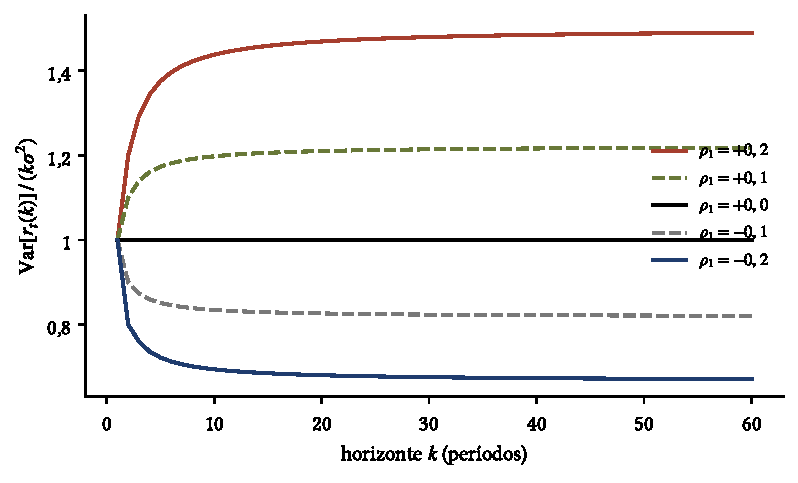
\includegraphics[width=0.72\linewidth]{graficos/cap01_fig_razonvar.pdf}
\caption{Cociente entre la varianza del rendimiento de $k$ períodos y la que predice la regla de la raíz del tiempo ($k\sigma^2$), cuando $\rho_j=\rho_1^{\,j}$. Sin autocorrelación el cociente es 1 en todos los horizontes. Con $\rho_1=0{,}2$ la varianza de largo plazo es un 50\,\% mayor; con $\rho_1=-0{,}2$ es un tercio menor. El límite es $(1+\rho_1)/(1-\rho_1)$.}
\label{fig:razonvar}
\end{figure}


\subsection{Media aritmética y media geométrica}

Con una muestra de $T$ rendimientos simples $R_1,\dots,R_T$ hay dos maneras naturales de promediar:
la media aritmética $A=\frac1T\sum_tR_t$ y la media geométrica $G$, definida por
$(1+G)^T=\prod_t(1+R_t)$, que es la tasa constante que habría producido el mismo valor final.

\begin{proposicion}\label{prop:amgm}
Se cumple $G\le A$, con igualdad si y solo si todos los $R_t$ son iguales. Además, a segundo orden,
\[
  G\approx A-\tfrac12\,s^2,\qquad s^2=\frac1T\sum_{t=1}^T(R_t-A)^2 .
\]
\end{proposicion}

\begin{proof}
Tomamos logaritmos en la definición de $G$ y aplicamos la desigualdad de Jensen a la función cóncava
$\ln$, con pesos $1/T$:
\begin{align*}
  (1+G)^T        &= \prod_{t=1}^T(1+R_t)\\
  T\ln(1+G)      &= \sum_{t=1}^T\ln(1+R_t)\\
  \ln(1+G)       &= \frac1T\sum_{t=1}^T\ln(1+R_t)\\
                 &\le \ln\Bigl(\frac1T\sum_{t=1}^T(1+R_t)\Bigr) && \text{(Jensen)}\\
                 &= \ln(1+A).
\end{align*}
Como el logaritmo es creciente, $G\le A$, con igualdad solo si todos los $R_t$ son iguales.

Para la aproximación, usamos $\ln(1+x)\approx x-\tfrac12x^2$ (Proposición~\ref{prop:taylor}) en ambos
lados de la tercera línea. A la izquierda, $\ln(1+G)\approx G-\tfrac12G^2$. A la derecha,
\begin{align*}
  \frac1T\sum_t\ln(1+R_t) &\approx \frac1T\sum_t\Bigl(R_t-\tfrac12R_t^2\Bigr)\\
                          &= A-\tfrac12\cdot\frac1T\sum_tR_t^2\\
                          &= A-\tfrac12\,(s^2+A^2),
\end{align*}
donde usamos $\frac1T\sum_tR_t^2=s^2+A^2$. Igualando ambos lados:
\begin{align*}
  G-\tfrac12G^2 &\approx A-\tfrac12A^2-\tfrac12s^2\\
  G             &\approx A-\tfrac12s^2+\tfrac12\,(G^2-A^2)\\
  G             &\approx A-\tfrac12s^2.
\end{align*}
En la última línea eliminamos $\tfrac12(G^2-A^2)$: como $G$ y $A$ difieren en términos de segundo orden,
$G^2$ y $A^2$ difieren en términos de tercer orden.
\end{proof}

La diferencia entre ambas medias no es un detalle técnico. La media aritmética es el mejor estimador del
rendimiento \emph{esperado de un período}; la geométrica describe el crecimiento \emph{efectivo} de una
inversión mantenida varios períodos. En activos volátiles, como las acciones mineras, la brecha
$s^2/2$ puede ser de varios puntos porcentuales al año.

\subsection{Rendimientos lognormales}

Un supuesto clásico, que el Capítulo~2 pondrá a prueba con datos, es que el rendimiento logarítmico es
normal.

\begin{proposicion}\label{prop:lognormal}
Si $r_t\sim N(\mu,\sigma^2)$, entonces $1+R_t=e^{r_t}$ tiene distribución lognormal, con
\[
  \E[1+R_t]=e^{\mu+\sigma^2/2},\qquad \operatorname{Mediana}(1+R_t)=e^{\mu},\qquad
  \Var[R_t]=e^{2\mu+\sigma^2}\bigl(e^{\sigma^2}-1\bigr).
\]
\end{proposicion}

\begin{proof}
Calculamos $\E[e^{a\,r_t}]$ para un número real $a$:
\[
  \E[e^{a r_t}]=\int_{-\infty}^{\infty}\frac{1}{\sqrt{2\pi}\,\sigma}
  \exp\Bigl(ax-\frac{(x-\mu)^2}{2\sigma^2}\Bigr)dx .
\]
Completamos el cuadrado en el exponente, escribiendo $ax=a(x-\mu)+a\mu$:
\begin{align*}
  ax-\frac{(x-\mu)^2}{2\sigma^2}
    &= -\frac{(x-\mu)^2-2a\sigma^2(x-\mu)}{2\sigma^2}+a\mu\\
    &= -\frac{(x-\mu)^2-2a\sigma^2(x-\mu)+a^2\sigma^4}{2\sigma^2}+\frac{a^2\sigma^4}{2\sigma^2}+a\mu\\
    &= -\frac{(x-\mu-a\sigma^2)^2}{2\sigma^2}+a\mu+\frac{a^2\sigma^2}{2}.
\end{align*}
Sustituyendo en la integral:
\begin{align*}
  \E[e^{a r_t}]
    &= e^{a\mu+a^2\sigma^2/2}\int_{-\infty}^{\infty}\frac{1}{\sqrt{2\pi}\,\sigma}
       \exp\Bigl(-\frac{(x-\mu-a\sigma^2)^2}{2\sigma^2}\Bigr)dx\\
    &= e^{a\mu+a^2\sigma^2/2}\cdot1\\
    &= e^{a\mu+a^2\sigma^2/2},
\end{align*}
porque la integral es la de una densidad $N(\mu+a\sigma^2,\sigma^2)$. Con $a=1$ y $a=2$:
\begin{align*}
  \E[1+R_t]     &= \E[e^{r_t}] = e^{\mu+\sigma^2/2},\\
  \E[(1+R_t)^2] &= \E[e^{2r_t}] = e^{2\mu+2\sigma^2}.
\end{align*}
Para la varianza:
\begin{align*}
  \Var[R_t] &= \Var[1+R_t]\\
            &= \E[(1+R_t)^2]-\bigl(\E[1+R_t]\bigr)^2\\
            &= e^{2\mu+2\sigma^2}-e^{2\mu+\sigma^2}\\
            &= e^{2\mu+\sigma^2}\bigl(e^{\sigma^2}-1\bigr).
\end{align*}
Por último, la mediana se conserva por transformaciones crecientes: como la mediana de $r_t$ es $\mu$, la
de $e^{r_t}$ es $e^{\mu}$.
\end{proof}

La proposición muestra que la media de los rendimientos simples supera a la mediana en el factor
$e^{\sigma^2/2}$: la distribución de $R_t$ es asimétrica a la derecha aunque la de $r_t$ sea simétrica.
Es la versión poblacional de la Proposición~\ref{prop:amgm}. La Figura~\ref{fig:lognormal} muestra ambas cosas: al crecer $\sigma$ la densidad se vuelve más asimétrica, y la media se aleja de la mediana.
\begin{figure}[ht]
\centering
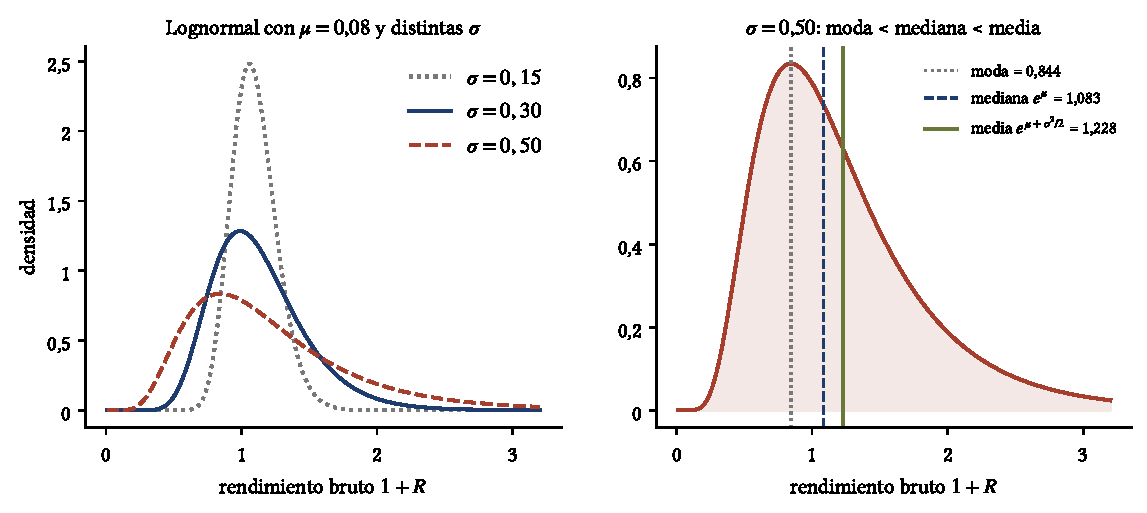
\includegraphics[width=\linewidth]{graficos/cap01_fig_lognormal.pdf}
\caption{Distribución lognormal del rendimiento bruto $1+R=e^{r}$ con $r\sim N(\mu,\sigma^2)$. Izquierda: con más volatilidad la densidad se aplana y se alarga hacia la derecha; la masa se desplaza a valores bajos, pero la cola derecha se extiende. Derecha: con $\sigma=0{,}50$ la moda ($e^{\mu-\sigma^2}$), la mediana ($e^{\mu}$) y la media ($e^{\mu+\sigma^2/2}$) quedan claramente separadas (Proposición~\ref{prop:lognormal}).}
\label{fig:lognormal}
\end{figure}


% ---------------------------------------------------------------------
\section{Datos reales: fuentes, calendarios y sincronización}\label{sec:datos}
% ---------------------------------------------------------------------

\subsection{Fuentes usadas en este capítulo}

\begin{table}[ht]
\centering\footnotesize
\begin{tabularx}{\linewidth}{@{}lXlrll@{}}
\toprule
Serie & Descripción & Fuente & $n$ & Primer dato & Último dato \\
\midrule
\texttt{PD38026MD} & Índice S\&P/BVL Perú General (soles) & BCRPData & 3013 & 14\,794,32 & 54\,971,46 \\
\texttt{PD04638PD} & Tipo de cambio interbancario, venta (S/ por US\$) & BCRPData & 2952 & 2,9830 & 3,4487 \\
\texttt{BAP} & Credicorp Ltd. (NYSE, dólares) & Yahoo Finance & 2981 & 160,18 & 347,93 \\
\texttt{SCCO} & Southern Copper Corp. (NYSE, dólares)$^{a}$ & Yahoo Finance & 2981 & 26,09 & 167,27 \\
\texttt{BVN} & Cía. de Minas Buenaventura (NYSE, ADR) & Yahoo Finance & 2981 & 9,56 & 27,99 \\
\texttt{EPU} & iShares MSCI Peru ETF (dólares) & Yahoo Finance & 2981 & 31,96 & 80,41 \\
\texttt{\^{}GSPC} & Índice S\&P 500 & Yahoo Finance & 2981 & 2\,058,90 & 7\,376,86 \\
\texttt{PEN=X} & Tipo de cambio USD/PEN, último dato del mes & Yahoo Finance & 144 & 2,9930 & 3,4398 \\
\bottomrule
\end{tabularx}
\caption{Series del Capítulo 1 (archivos de \texttt{datos/peru/}). El primer dato es del 31 de diciembre
de 2014 en todas las series; el último, del 5 de noviembre de 2026 (BCRP), del 6 de noviembre de 2026
(acciones e índices de Yahoo) y del 9 de noviembre de 2026 (\texttt{PEN=X}). Descarga: 8 y 9 de noviembre
de 2026. Para las acciones se guardan el cierre y el cierre ajustado. $^{a}$Cierre ya ajustado por los
dividendos en acciones de 2024--2026, que Yahoo registra como desdoblamientos.}
\label{tab:fuentes1}
\end{table}

Los metadatos que devuelve la API del BCRP describen \texttt{PD04638PD} como ``Tipo de cambio -- TC
Interbancario (S/ por US\$) -- Venta''. El índice de la BVL se toma del BCRP y no de Yahoo Finance porque
el símbolo \texttt{\^{}SPBLPGPT} ya no devuelve datos en Yahoo. Al revisar las series aparecieron tres
problemas que se tratan en los ejercicios: (i) el 21 de junio de 2024 el BCRP registra el índice en
22\,521,03, entre 29\,857,57 y 30\,058,66, un dato claramente erróneo que se elimina; (ii) hasta 2020 el
BCRP repite el valor del día anterior en los feriados peruanos (54 rendimientos exactamente iguales a cero),
y desde 2021 los deja como ``n.d.''; (iii) Yahoo Finance registra dos veces el dividendo de Credicorp de
abril de 2020 (Ejercicio~\ref{ej:dividendos}).

\subsection{Problemas prácticos que hay que resolver antes de modelar}

\paragraph{Calendarios de negociación distintos.} La BVL y la Bolsa de Nueva York no cierran los mismos
días: la BVL cierra en feriados peruanos (por ejemplo, el 28 y 29 de julio) y Nueva York en feriados
estadounidenses (por ejemplo, el Día de Acción de Gracias). El BCRP publica el tipo de cambio en días
hábiles del Perú. Al unir series hay dos alternativas: (i) quedarse solo con las fechas comunes
(\emph{intersección}), que pierde observaciones pero no inventa datos; o (ii) completar los faltantes con
el último precio conocido (\emph{arrastre hacia adelante}), que conserva fechas pero genera rendimientos
iguales a cero el día del feriado y un rendimiento acumulado al día siguiente. La segunda opción reduce
artificialmente la varianza diaria y sesga las correlaciones. En este libro usaremos la intersección,
salvo que se indique lo contrario.

\paragraph{Horarios de cierre.} Aunque dos series tengan la misma fecha, sus cierres pueden ocurrir a
horas distintas. El tipo de cambio interbancario del BCRP corresponde al cierre del mercado cambiario
local, que no coincide con el cierre de la Bolsa de Nueva York. Esta asincronía tiene poco efecto en
rendimientos mensuales, pero en datos diarios puede inducir correlaciones rezagadas espurias.

\paragraph{Precios ajustados que cambian.} Cada nuevo dividendo modifica \emph{toda} la historia de
precios ajustados anterior (Proposición~\ref{prop:ajuste}). Por eso dos descargas en fechas distintas
dan niveles de precios ajustados diferentes, aunque los rendimientos sean los mismos. Siempre guardamos
una copia de los datos descargados (carpeta \texttt{datos/}) y registramos la fecha de descarga.

\paragraph{Errores y valores extremos.} Las series públicas contienen ocasionalmente precios repetidos,
días sin negociación registrados con volumen cero o saltos que corresponden a eventos corporativos. Un
rendimiento diario extremo debe verificarse antes de eliminarlo: en finanzas, los valores extremos suelen
ser información (Capítulo~2), no errores.

% ---------------------------------------------------------------------
\section{Ejercicios resueltos}
% ---------------------------------------------------------------------

\begin{ejresuelto}{Dividendos de Credicorp: precio de cierre frente a precio ajustado}\label{ej:dividendos}
\enunciado Con los precios diarios de Credicorp (\texttt{BAP}) desde 2015: (a) identifique las fechas
ex-dividendo a partir del cociente entre el precio ajustado y el de cierre; (b) recupere el monto de cada
dividendo con la ecuación \eqref{eq:factor} y verifique la Proposición~\ref{prop:ajuste}; (c) compare el
rendimiento acumulado con precios de cierre y con precios ajustados y explique la diferencia.

\solucion
\paso{Paso 1. Idea.} Sea $c_t=P^a_t/P_t$ el cociente entre el precio ajustado y el de cierre. Por la regla
de ajuste, $c_t$ es constante entre dos eventos y salta en cada fecha ex-dividendo:
\begin{align*}
  c_{t-1} &= c_t\,f_t\\
  f_t     &= \frac{c_{t-1}}{c_t}\\
  1-\frac{D_t}{P_{t-1}} &= \frac{c_{t-1}}{c_t} && \text{(por \eqref{eq:factor})}\\
  D_t     &= \Bigl(1-\frac{c_{t-1}}{c_t}\Bigr)P_{t-1}.
\end{align*}
\paso{Paso 2. Verificación.} Con $D_t$ recuperado se calculan, en cada fecha ex-dividendo,
\begin{align*}
  R^{\mathrm{tot}}_t       &= \frac{P_t+D_t}{P_{t-1}}-1,\\
  R^{a}_t                  &= \frac{P^{a}_t}{P^{a}_{t-1}}-1,\\
  R^{a}_t-R^{\mathrm{tot}}_t &= \frac{d_t}{1-d_t}\,R^{\mathrm{tot}}_t,
\end{align*}
y se comprueba que la última igualdad (Proposición~\ref{prop:ajuste}) se cumple.

\paso{Paso 3. Cálculo.} Los programas detectan los saltos de $c_t$ mayores que $10^{-4}$, recuperan
$D_t$ y $d_t$, verifican \eqref{eq:difajuste} y calculan el rendimiento acumulado.

\codigoweb{cap01_ej01}
\salidaR{cap01_ej01_R.txt}
\lectura{cap01_ej01}

\RvsPy Ambos lenguajes dan los mismos 17 eventos y los mismos montos. La diferencia de $1{,}41\times
10^{-6}$ fuera de los eventos no es un error de la regla de ajuste: proviene de que el precio ajustado
se guardó con cuatro decimales.

\paso{Paso 4. Comparación con los dividendos anunciados.} La página de relación con inversionistas de
Credicorp publica el monto en dólares de cada dividendo. La Tabla~\ref{tab:divbap} compara los que
figuran ahí con los recuperados.

\begin{table}[H]
\centering\small
\begin{tabular}{@{}lrrl@{}}
\toprule
Fecha ex (Yahoo) & $D_t$ recuperado & Anunciado (US\$) & Fecha de registro \\
\midrule
17-abr-2015 & 2,187 & 2,1900 & 21-abr-2015 \\
14-abr-2016 & 2,316 & 2,3200 & 18-abr-2016 \\
08-abr-2020 & 8,803 & \multirow{2}{*}{8,8026} & \multirow{2}{*}{13-abr-2020} \\
09-abr-2020 & 8,803 & & \\
14-set-2021 & 1,209 & 1,2104 & 15-set-2021 \\
19-may-2022 & 3,994 & 3,9936 & 20-may-2022 \\
18-may-2023 & 6,775 & 6,7749 & 19-may-2023 \\
17-may-2024 & 9,288 & 9,2875 & 20-may-2024 \\
23-set-2024 & 2,917 & 2,9167 & 23-set-2024 \\
19-may-2025 & 11,011 & 11,0162 & 19-may-2025 \\
18-may-2026 & 14,276 & 14,6379 & 18-may-2026 \\
\bottomrule
\end{tabular}
\caption{Dividendos de Credicorp: montos recuperados del precio ajustado y montos anunciados por la
empresa (que los declara en soles y publica su equivalente en dólares). Los años 2017--2019 no figuran en
la página consultada.}
\label{tab:divbap}
\end{table}

Los montos coinciden hasta el redondeo, con dos excepciones. En 2026 Yahoo usa un monto en dólares
menor (14,276 frente a 14,638), probablemente por convertir los soles con otro tipo de cambio. En 2020 la
empresa pagó \emph{un} dividendo de S/\,30 (US\$\,8,8026), pero Yahoo lo registra dos veces, el 8 y el 9 de
abril: el precio ajustado anterior a esa fecha está multiplicado por un factor de más, $0{,}9335$, y el
rendimiento total del período queda sobrestimado. Lo mismo podría ocurrir con los dos registros
consecutivos de abril de 2017 (0,378 y 3,738), que no se pudieron contrastar.

\begin{figure}[H]
\centering
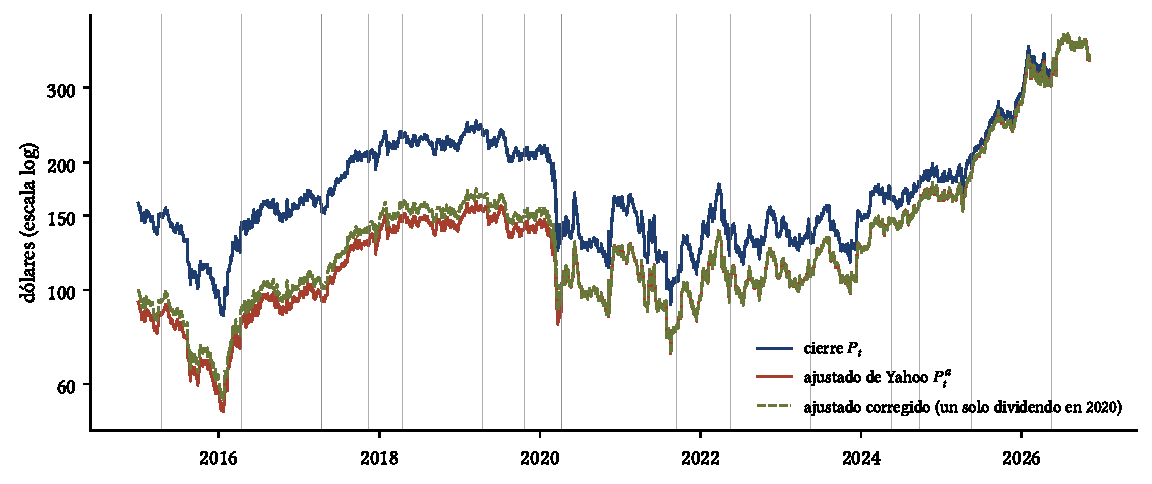
\includegraphics[width=\linewidth]{graficos/cap01_fig_dividendos.pdf}
\caption{Credicorp (\texttt{BAP}), 2015--2026: precio de cierre, precio ajustado de Yahoo Finance y
precio ajustado corregido (un solo dividendo en 2020), en escala logarítmica. Las líneas verticales marcan
las fechas ex-dividendo. Las tres series coinciden después del último dividendo (18 de mayo de 2026).}
\label{fig:divbap}
\end{figure}

\begin{conclusion}
El cociente $c_t$ recupera exactamente los dividendos y la Proposición~\ref{prop:ajuste} se cumple con
error de $3\times10^{-16}$. Sin dividendos, la acción rindió 117,2\,\% entre diciembre de 2014 y noviembre
de 2026 (6,8\,\% anual); con los dividendos reinvertidos rindió 247,0\,\% (11,1\,\% anual). Los dividendos
explican, por tanto, cerca de 4,3 puntos de rentabilidad anual. Si se usa sin revisar el precio ajustado
de Yahoo, el rendimiento acumulado sería 271,8\,\%: un error de descarga de 25 puntos.
\end{conclusion}
\end{ejresuelto}

\begin{ejresuelto}{Rendimientos simples y logarítmicos del mercado peruano y del S\&P 500}\label{ej:logsimple}
\enunciado Con el índice S\&P/BVL Perú General y el S\&P 500: (a) calcule los rendimientos diarios
simples y logarítmicos; (b) verifique que $r_t\le R_t$ en todas las fechas y encuentre el día con mayor
diferencia; (c) agregue a rendimientos mensuales y anuales de dos formas: sumando logaritmos y
multiplicando rendimientos brutos, y compruebe que coinciden (Proposiciones~\ref{prop:multi}
y~\ref{prop:aditiva}).

\solucion
\paso{Paso 1. Datos.} Usamos el índice de la BVL que publica el BCRP (\texttt{PD38026MD}), tras eliminar
el dato erróneo del 21 de junio de 2024, y el S\&P 500 de Yahoo Finance. Si no se elimina ese dato, la
serie muestra un rendimiento logarítmico de $-28{,}2$\,\% seguido de otro de $+28{,}9$\,\%, que dominarían
cualquier estadístico.

\paso{Paso 2. Qué esperar.} Como $r_t=\ln(1+R_t)$ y $\ln(1+x)\le x$, la diferencia
\begin{align*}
  R_t-r_t &= R_t-\ln(1+R_t)\\
          &= \tfrac12R_t^2-\tfrac13R_t^3+\cdots
\end{align*}
es siempre no negativa y crece con $|R_t|$: la mayor diferencia debe aparecer en el día de mayor
movimiento.

\codigoweb{cap01_ej02}
\salidaR{cap01_ej02_R.txt}
\lectura{cap01_ej02}

\RvsPy En R se agrupa con \texttt{tapply} y \texttt{format(fecha, "\%Y-\%m")}; en Python con
\texttt{pd.Grouper}. Las diferencias entre la suma de logaritmos y el logaritmo del producto son del orden
de $10^{-15}$ en ambos: son errores de redondeo de la aritmética de punto flotante, no diferencias de
método.

\begin{figure}[H]
\centering
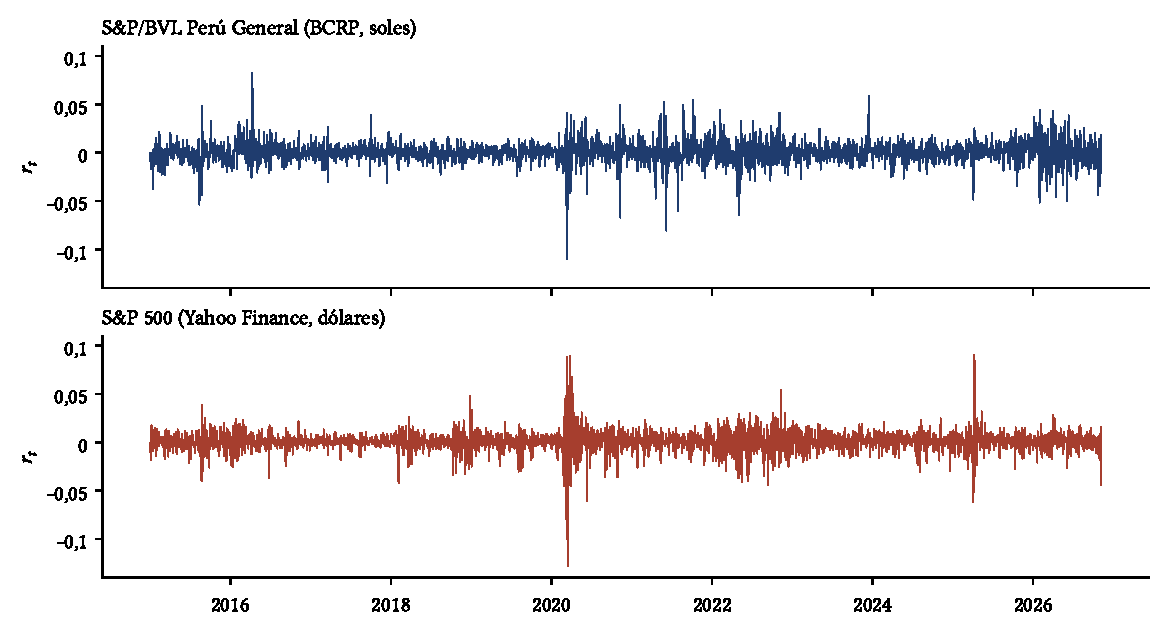
\includegraphics[width=\linewidth]{graficos/cap01_fig_logsimple.pdf}
\caption{Rendimientos logarítmicos diarios del índice S\&P/BVL Perú General (BCRP) y del S\&P 500
(Yahoo Finance), enero de 2015 a noviembre de 2026.}
\label{fig:logsimple-datos}
\end{figure}

\begin{conclusion}
En las 3011 fechas del índice de la BVL y las 2980 del S\&P 500 se cumple $r_t\le R_t$. La mayor
diferencia ocurre en la caída de marzo de 2020: 0,58 puntos porcentuales el 12 de marzo en la BVL
($R_t=-10{,}42$\,\%, $r_t=-11{,}01$\,\%) y 0,78 puntos el 16 de marzo en el S\&P 500. Las Proposiciones
\ref{prop:multi} y \ref{prop:aditiva} se verifican en las 143 agregaciones mensuales y las 12 anuales.
Ambos índices tienen media y volatilidad diarias muy parecidas (0,044\,\% y 1,1\,\%), pero sus
trayectorias anuales difieren mucho: la BVL cayó 33\,\% en 2015 y subió 58\,\% en 2016 y 50\,\% en 2025.
Recuérdese que el índice de la BVL está en soles y el S\&P 500 en dólares.
\end{conclusion}
\end{ejresuelto}

\begin{ejresuelto}{¿Cuánto ganó en soles un inversionista peruano en Southern Copper?}\label{ej:soles}
\enunciado Un inversionista peruano mide su riqueza en soles. (a) Construya el valor en soles de una
acción de \texttt{SCCO} con el tipo de cambio interbancario del BCRP; (b) descomponga el rendimiento
logarítmico anual en soles en la parte de la acción y la parte del tipo de cambio
(Proposición~\ref{prop:moneda}); (c) repita con el tipo de cambio \texttt{PEN=X} de Yahoo Finance y
compare: ¿cambian las conclusiones por la fuente del tipo de cambio?

\solucion
\paso{Paso 1. Planteamiento.} Con $P_t$ el precio ajustado en dólares y $S_t$ el tipo de cambio, el valor
en soles es $V_t=P_tS_t$. Por la Proposición~\ref{prop:moneda}, en cada año
\begin{align*}
  r^{\mathrm{S/}}_t &= \ln V_t-\ln V_{t-1}\\
                    &= (\ln P_t-\ln P_{t-1})+(\ln S_t-\ln S_{t-1})\\
                    &= r^{\$}_t+\Delta\ln S_t .
\end{align*}
Tomamos el último dato disponible de cada fin de año, de 2014 a 2025, y el del 30 de octubre de 2026 como
último corte (fila 2026*), porque \texttt{PEN=X} se guardó con un dato por mes.

\codigoweb{cap01_ej03}
\salidaR{cap01_ej03_R.txt}
\lectura{cap01_ej03}

\RvsPy La función \texttt{ultimo} hace lo mismo en ambos lenguajes: busca el último dato con fecha menor o
igual al corte. Así se resuelve que el 31 de diciembre no sea día hábil en algunos años y que cada serie
tenga su propio calendario.

\begin{figure}[H]
\centering
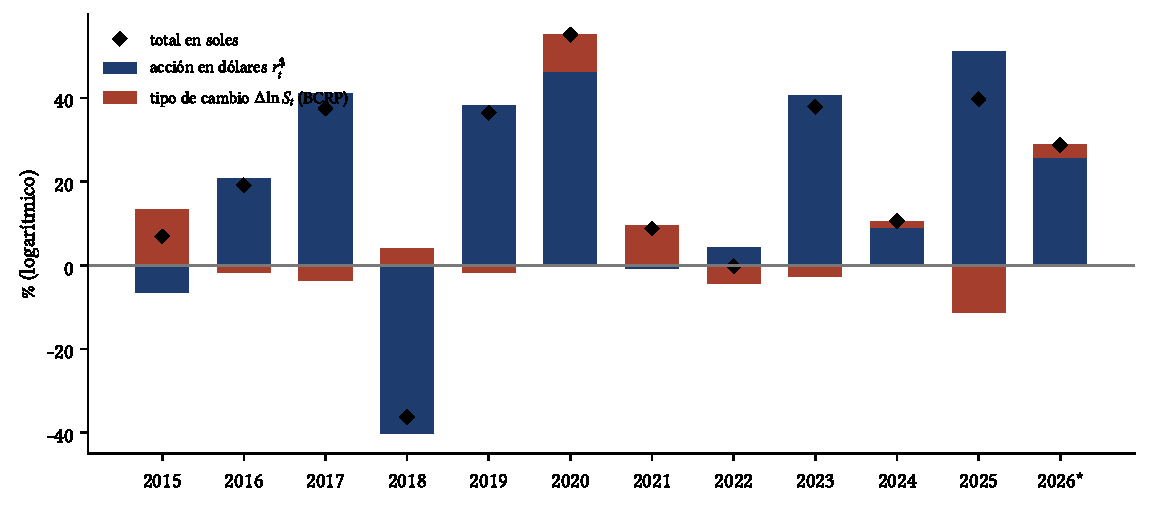
\includegraphics[width=\linewidth]{graficos/cap01_fig_soles.pdf}
\caption{Rendimiento logarítmico anual de \texttt{SCCO} en soles: parte de la acción en dólares y parte
del tipo de cambio interbancario del BCRP. Los rombos marcan el total en soles. 2026*: hasta el 30 de
octubre.}
\label{fig:soles}
\end{figure}

\begin{conclusion}
Entre diciembre de 2014 y octubre de 2026, una acción de Southern Copper rindió 229,7 puntos logarítmicos
en dólares (894\,\% simple) y 244,7 en soles (1055\,\%); los 15 puntos de diferencia son la depreciación
acumulada del sol según el BCRP. El tipo de cambio pesa poco frente a la acción, salvo en años
concretos: en 2015 la depreciación del sol (13,4 puntos) convirtió una pérdida de $-6{,}5$ en dólares en
una ganancia de 6,9 en soles, y en 2025 la apreciación ($-11{,}3$ puntos) le quitó a un inversionista en
soles una cuarta parte de la ganancia. Con \texttt{PEN=X} de Yahoo las conclusiones cualitativas no
cambian, pero las cifras de un año pueden diferir hasta en 2,7 puntos (2015) y el signo de la variación
del tipo de cambio cambia en 2024. Para trabajos sobre el Perú conviene usar el tipo de cambio oficial
del BCRP.
\end{conclusion}
\end{ejresuelto}

\begin{ejresuelto}{Un portafolio de acciones peruanas: suma simple frente a suma logarítmica}\label{ej:portafolio}
\enunciado Considere un portafolio con un tercio del valor en \texttt{BAP}, \texttt{SCCO} y \texttt{BVN},
rebalanceado al inicio de cada mes. (a) Calcule su rendimiento mensual exacto con la
Proposición~\ref{prop:portafolio}; (b) calcule la aproximación $\sum_iw_ir_{i,t}$ y verifique la
Proposición~\ref{prop:logport}; (c) mida el error de aproximación y su relación con la dispersión de los
rendimientos entre las tres acciones; (d) compare con la estrategia sin rebalanceo.

\solucion
\paso{Paso 1. Qué esperar.} Sea $\bar r_t=\sum_iw_ir_{i,t}$. Una expansión de segundo orden de
$e^{r_{i,t}}$ alrededor de $\bar r_t$ da
\begin{align*}
  \sum_iw_ie^{r_{i,t}} &\approx e^{\bar r_t}\sum_iw_i\Bigl[1+(r_{i,t}-\bar r_t)+\tfrac12(r_{i,t}-\bar r_t)^2\Bigr]\\
                       &= e^{\bar r_t}\Bigl[1+\tfrac12\sigma^2_{t}\Bigr],\qquad
                          \sigma^2_t\equiv\sum_iw_i(r_{i,t}-\bar r_t)^2,\\
  r_{p,t}-\bar r_t     &\approx \ln\bigl(1+\tfrac12\sigma^2_t\bigr)\\
                       &\approx \tfrac12\sigma^2_t .
\end{align*}
El error de la aproximación debe ser no negativo (Proposición~\ref{prop:logport}) y aproximadamente igual
a la mitad de la varianza transversal de los rendimientos.

\paso{Paso 2. Datos.} Precios ajustados de Yahoo, con la corrección del dividendo duplicado de Credicorp
(Ejercicio~\ref{ej:dividendos}), y último precio de cada mes. El último mes (noviembre de 2026) es parcial.

\codigoweb{cap01_ej04}
\salidaR{cap01_ej04_R.txt}
\lectura{cap01_ej04}

\RvsPy El producto matricial (\texttt{\%*\%} en R, \texttt{@} en Python) calcula $\sum_iw_iR_{i,t}$ para
todos los meses a la vez. Para la varianza transversal se usa divisor $N$ (no $N-1$) en ambos lenguajes,
porque así está definida $\sigma^2_t$ en el Paso~1.

\begin{figure}[H]
\centering
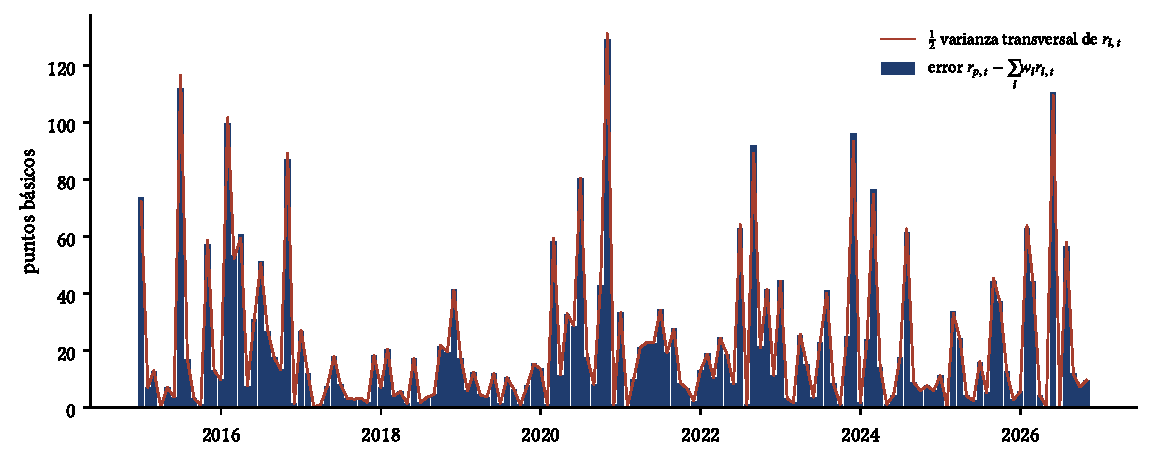
\includegraphics[width=\linewidth]{graficos/cap01_fig_portafolio.pdf}
\caption{Error mensual de aproximar el rendimiento logarítmico del portafolio por
$\sum_iw_ir_{i,t}$ (barras) y la mitad de la varianza transversal de los tres rendimientos (línea), en
puntos básicos.}
\label{fig:portafolio}
\end{figure}

\begin{conclusion}
El error es positivo en los 143 meses, como exige la Proposición~\ref{prop:logport}. En promedio es de
21,7 puntos básicos al mes, pero llega a 129 en noviembre de 2020, cuando las tres acciones se movieron de
forma muy distinta. La regresión del error sobre la varianza transversal da una pendiente de 0,498,
casi exactamente el $\tfrac12$ del Paso~1. Acumulado en 12 años, el error suma 31 puntos logarítmicos:
la aproximación es aceptable para un mes, pero no para medir el rendimiento de largo plazo. El rebalanceo
mensual convirtió un dólar en 6,45; sin rebalancear se habría llegado a 5,39, y Southern Copper habría
pasado a representar el 59\,\% del portafolio.
\end{conclusion}
\end{ejresuelto}

\begin{ejresuelto}{Media aritmética, media geométrica y anualización}\label{ej:anualizar}
\enunciado Con los rendimientos anuales de \texttt{BVN}, \texttt{EPU} y el S\&P 500: (a) calcule las
medias aritmética y geométrica y verifique la aproximación $G\approx A-s^2/2$
(Proposición~\ref{prop:amgm}); (b) anualice la volatilidad diaria con la raíz del tiempo y compárela con
la volatilidad de los rendimientos anuales observados; (c) cuente cuántos días de negociación por año
tiene cada serie y discuta si 252 es adecuado.

\solucion
\paso{Paso 1. Datos.} Usamos los años completos 2015--2025 ($T=11$). Para \texttt{BVN} y \texttt{EPU}
se usa el precio ajustado (rendimiento total); para el S\&P 500, el índice de precios. La volatilidad
diaria se calcula con rendimientos logarítmicos y se anualiza de dos formas: con $\sqrt{252}$ y con la
raíz del número promedio de días observados por año.

\codigoweb{cap01_ej05}
\salidaR{cap01_ej05_R.txt}
\lectura{cap01_ej05}

\RvsPy En la media y la varianza de la parte (a) se usa divisor $T$, como en la
Proposición~\ref{prop:amgm}; en las desviaciones estándar de la parte (b), divisor $T-1$ (\texttt{sd} en
R y \texttt{std} en pandas). Ambos programas dan las mismas cifras.

\begin{figure}[H]
\centering
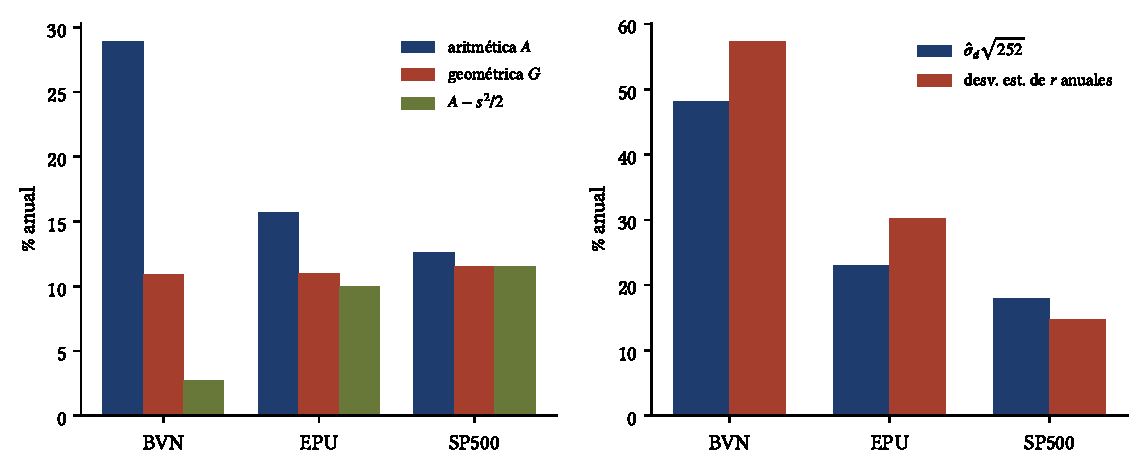
\includegraphics[width=\linewidth]{graficos/cap01_fig_anualizar.pdf}
\caption{Izquierda: medias aritmética y geométrica de los rendimientos anuales 2015--2025 y la
aproximación $A-s^2/2$. Derecha: volatilidad diaria anualizada con $\sqrt{252}$ y desviación estándar
de los rendimientos anuales observados.}
\label{fig:anualizar}
\end{figure}

\begin{conclusion}
(a) En las tres series $G<A$. Para el S\&P 500 la aproximación $G\approx A-s^2/2$ es excelente (11,52
frente a 11,54\,\%) y para \texttt{EPU} razonable (10,00 frente a 11,02\,\%). Para \texttt{BVN} falla
($2{,}72$ frente a $10{,}88$\,\%): con rendimientos anuales de $-55$\,\%, $+164$\,\% o $+148$\,\% los
términos de tercer y cuarto orden que la aproximación omite ya no son pequeños. La media aritmética de
\texttt{BVN} (28,9\,\%) exagera mucho lo que ganó un inversionista que mantuvo la acción (10,9\,\% anual).
(b) Anualizar con $\sqrt{252}$ o con el número de días observados da prácticamente lo mismo. La
volatilidad de los rendimientos anuales observados es mayor que la diaria anualizada en \texttt{BVN} y
\texttt{EPU}, y menor en el S\&P 500. La regla de la raíz del tiempo supone rendimientos independientes;
con solo 11 años, sin embargo, la desviación estándar anual es muy imprecisa. (c) Nueva York tuvo entre 250
y 253 días de negociación por año, así que 252 es adecuado. El BCRP publica 260--261 datos por año hasta
2020, porque repite el valor en los feriados peruanos, y 245--251 desde 2021. Para la BVL, entonces, hay
que contar los días con negociación efectiva y no los días con dato.
\end{conclusion}
\end{ejresuelto}

% ---------------------------------------------------------------------
\section{Ejercicios propuestos}
% ---------------------------------------------------------------------

\begin{enumerate}[label=\textbf{\thechapter.\arabic*},leftmargin=*,itemsep=6pt]
  \item\label{prop:ejsplit} Demuestre la Proposición~\ref{prop:split}: si en $t$ hay un desdoblamiento
  $k\!:\!1$, el precio de cierre cae aproximadamente a $P_{t-1}/k$, y los precios anteriores se
  multiplican por $1/k$, entonces $P^a_t/P^a_{t-1}$ es igual al cociente entre el valor de las $k$
  acciones en $t$ y el de la acción original en $t-1$.
  \textit{Pista: el accionista tiene $k$ acciones en $t$ y una en $t-1$.}

  \item\label{prop:ejasimetria} Demuestre que, para $0<x<1$, la brecha entre el rendimiento simple y el
  logarítmico es mayor para una pérdida que para una ganancia del mismo tamaño:
  $\bigl[-x-\ln(1-x)\bigr]>\bigl[x-\ln(1+x)\bigr]$. Compruebe los valores $0{,}193$ y $0{,}095$ de la
  Figura~\ref{fig:logsimple} para $x=0{,}5$.
  \textit{Pista: estudie $g(x)=-2x-\ln(1-x)+\ln(1+x)$ y su derivada $g'(x)=2x^2/(1-x^2)$.}

  \item\label{prop:ejcorto} Muestre que la desigualdad de la Proposición~\ref{prop:logport} puede
  invertirse con posiciones cortas. \textit{Respuesta: con $w=(2,-1)$, $r_1=0$ y $r_2=\ln 1{,}5$,
  se obtiene $r_p=\ln 0{,}5=-0{,}693<\sum_iw_ir_i=-\ln1{,}5=-0{,}405$.}

  \item Suponga que $\rho_j=\phi^{\,j}$ con $|\phi|<1$ (estructura de un proceso AR(1), Capítulo~6).
  Use la Proposición~\ref{prop:agregmom} para demostrar que
  \[
    \frac{\Var[r_t(k)]}{\sigma^2}=\frac{k(1-\phi^2)-2\phi(1-\phi^k)}{(1-\phi)^2},
  \]
  y que el cociente $\Var[r_t(k)]/(k\sigma^2)$ tiende a $(1+\phi)/(1-\phi)$ cuando $k\to\infty$.

  \item Si $r_t\sim N(\mu,\sigma^2)$, demuestre que $\E[R_t]>\operatorname{Mediana}(R_t)$ siempre que
  $\sigma>0$ y que el cociente $\E[1+R_t]/\operatorname{Mediana}(1+R_t)$ depende solo de $\sigma$.
  \textit{Respuesta: el cociente es $e^{\sigma^2/2}$.}

  \item Demuestre que el rendimiento real logarítmico de $k$ períodos es la suma de los rendimientos
  reales logarítmicos de cada período, y que esa propiedad no se cumple con la aproximación
  $R^{\mathrm{real}}_t\approx R_t-\pi_t$ en rendimientos simples.

  \item \emph{(Con datos.)} Con la inflación mensual de Lima Metropolitana (INEI, disponible también en
  BCRPData), calcule el rendimiento real anual del índice S\&P/BVL Perú General desde 2015 y compárelo
  con el nominal. ¿En qué años el rendimiento nominal fue positivo y el real negativo?

  \item \emph{(Con datos, investigación.)} Repita el Ejercicio~\ref{ej:soles} con \texttt{BVN} y con
  \texttt{EPU}. ¿En qué años la depreciación del sol protegió al inversionista peruano de las pérdidas en
  dólares?

  \item \emph{(Con datos, investigación.)} Identifique los días de 2024 en que la BVL estuvo cerrada y la
  Bolsa de Nueva York abierta, y viceversa. Calcule la correlación diaria entre el índice S\&P/BVL Perú
  General y \texttt{EPU} con intersección de fechas y con arrastre hacia adelante. ¿Cuál es mayor y por
  qué?
\end{enumerate}

% ---------------------------------------------------------------------
\section{Resumen de fórmulas}
% ---------------------------------------------------------------------

\begin{table}[H]
\centering\small
\begin{tabular}{@{}ll@{}}
\toprule
Concepto & Fórmula \\
\midrule
Rendimiento simple & $R_t=P_t/P_{t-1}-1$ \\
Rendimiento total & $R^{\mathrm{tot}}_t=(P_t+D_t)/P_{t-1}-1$ \\
Factor de ajuste por dividendo & $f_t=1-D_t/P_{t-1}$ \\
Rendimiento logarítmico & $r_t=\ln(1+R_t)=\ln P_t-\ln P_{t-1}$ \\
Agregación temporal & $1+R_t(k)=\prod_{j}(1+R_{t-j})$;\quad $r_t(k)=\sum_j r_{t-j}$ \\
Agregación entre activos & $R_{p,t}=\sum_iw_iR_{i,t}$;\quad $r_{p,t}=\ln\sum_iw_ie^{r_{i,t}}$ \\
Rendimiento en soles & $r^{\mathrm{S/}}_t=r^{\$}_t+\Delta\ln S_t$ \\
Rendimiento real & $r^{\mathrm{real}}_t=r_t-\ln(1+\pi_t)$ \\
Varianza de $k$ períodos & $\sigma^2\bigl[k+2\sum_{j=1}^{k-1}(k-j)\rho_j\bigr]$ \\
Media geométrica & $G\approx A-\tfrac12s^2$ \\
Momentos lognormales & $\E[1+R]=e^{\mu+\sigma^2/2}$;\quad $\operatorname{Med}(1+R)=e^{\mu}$ \\
\bottomrule
\end{tabular}
\caption{Fórmulas principales del Capítulo 1.}
\end{table}

\section*{Referencias}
\begin{itemize}[leftmargin=*]
  \item Campbell, J. Y., Lo, A. W. y MacKinlay, A. C. (1997). \emph{The Econometrics of Financial
        Markets}. Princeton University Press. Capítulo 1.
  \item Tsay, R. S. (2010). \emph{Analysis of Financial Time Series} (3.ª ed.). Wiley. Capítulo 1.
  \item Banco Central de Reserva del Perú. \emph{BCRPData: series estadísticas}.
        \url{https://estadisticas.bcrp.gob.pe}.
  \item Instituto Nacional de Estadística e Informática. \emph{Índice de precios al consumidor de Lima
        Metropolitana}. \url{https://www.inei.gob.pe}.
\end{itemize}
